\subsubsection{薄膜太陽電池ミッション(大野・坂本)}
薄膜太陽電池ミッションは,多機能膜展開ミッションの一つであり,展開膜上に配置された薄膜太陽電池の発電量を評価することを目的とする.要求としては,
\begin{itemize}
	\item 多機能膜展開後,I-V特性を測定する
	\item 薄膜太陽電池の温度を測定する
\end{itemize}
ということがあげられる.

\subsubsection*{薄膜太陽電池の設計}
\begin{figure}[H]
	\centering
	\includegraphics[scale=0.5]{03/fig/FM_TFSC.jpg}
	\caption{FM展開膜の薄膜太陽電池}
	\label{fig3-9-3-1}
\end{figure}
FMの薄膜太陽電池の配置図を図\ref{fig3-9-3-1}に示す.薄膜太陽電池は両端に電極があり,そこにフレキシブル導電糸をリベットで固定し,MDCへと接続している.サーミスタ(103JT-025,SEMITEC)は,薄膜太陽電池の裏側に配置している.設計の方針として,接着成分を膜上に載せないことがあげられる.これは,サカセさんからの要求であり,展開に影響がある可能性があるからである.

\subsubsection*{太陽電池IV特性}
CIGS太陽電池については,JAXAソーラーセイルWGがOKEANOSミッションへの搭載を検討する目的で購入したものを宇宙科学研究所の太陽電池を扱うグループに3つに切断していただいて東工大へ送っていただいた(2016年12月30日).
東工大へ送付前に,宇宙科学研究所にてIV特性およびElectroluminescenceの計測をして下さった.
東工大でも2018年6月3日に,松永研のソーラーシミュレータを用いて薄膜太陽電池のIV特性を計測した.
	\begin{figure}[H]
	\begin{tabular}{cc}
		\begin{minipage}[t]{0.5\hsize}
			\centering
			\includegraphics[width=1\textwidth]{03/fig/3-9-3-12.jpg}
		\end{minipage} &
		
		\begin{minipage}[t]{0.5\hsize}
			\centering
			\includegraphics[width=1\textwidth]{03/fig/3-9-3-13.png}
		\end{minipage}
	\end{tabular}	
			\caption{JAXAソーラーセイルWGによる薄膜太陽電池の切断}
\label{fig3-9-3-12}
\end{figure}
\begin{figure}[h]
			\centering
			\includegraphics[width=.5\textwidth]{03/fig/3-9-3-14.jpg}
	\caption{薄膜太陽電池のIV特性計測@東工大(2018年6月3日)}
	\label{fig3-9-3-14}
\end{figure}

\subsubsection*{各要素の選定過程}
\begin{itemize}
	\item [\textbf{サーミスタの配置}]
	サーミスタ自体はもともと本衛星の別の箇所で使用していたものを使用した.したがって,ここでは配置についてのみ記述する.要求する値は,発電する表温度である.
	しかし,薄膜太陽電池とサーミスタの接着方法はホットメルト接着剤を考えており,表側であると発電部に貼付することとなるので,発電量が減少する恐れもある.以上のことから.裏側の貼付が望ましいと考え,サーミスタを表側に貼付した場合と,裏側に貼付した場合について実験を行い,比較した.結果としては,双方間の発電特性の差は,誤差の範囲内であったため,サーミスタを裏側に貼付しても発電面の温度と同等な値が得られるので,裏側に貼付することとした.\\
	\item [\textbf{フレキシブル導電糸と薄膜太陽電池の接続方法}]
	当初は半田付けを予定していたが,半田付けをすると薄膜太陽電池の電極部の皮膜がはがれる事態となった.それにより,導電性接着剤(CHO-BOND 1030-55,太陽金網株式会社)を使用した.
	しかし,これであると,粘着成分を膜上に搭載することになるので,サカセさんより,リベットによる固定方法を提案していただいた.
	これは,薄膜太陽電池に穴を開け,フレキシブル導電糸を電極に半田付けし,ねじで固定する方法である.イメージ図を図\ref{fig3-9-3-2}に示す.\\
	\begin{figure}[H]
		\centering
		\includegraphics[scale=0.7]{03/fig/how_to_fix_TFSC.jpg}
		\caption{薄膜太陽電池とフレキシブル導電糸の接続方法}
		\label{fig3-9-3-2}
	\end{figure}
	この設計でFMを製作したが,薄膜太陽電池に穴を開けるとき,ポンチであけていたが,薄膜太陽電池が裂ける可能性があるため,注意が必要である.(不要となった薄膜太陽電池を用いて何度も練習してから製作するのが望ましい.)\\
	\item [\textbf{配線}]
	配線で気をつけた点は2点ある.
	1つ目は電極付近をたるませることである.ねじで固定後の初めての展開実験で,展開衝撃により,フレキシブル導電糸に張力が加わり,薄膜太陽電池のねじ固定部が裂ける事態となった.これにより,フレキシブル導電糸のねじ固定部付近をたるませて配線することとした.
	2つ目は展開膜の折り目に沿って配線することである.折り目に沿わせることで,展開時に阻害しないようになる.
\end{itemize}

\subsubsection*{薄膜太陽電池の製作方法}
ここでは,FM展開膜の最終組立工程を記述する.\\
用意するもの:
薄膜太陽電池×2, サーミスタ×2, フレキシブル導電糸×8(薄膜太陽電池用×4,サーミスタ用×4:それぞれの長さは,展開膜上に配置し決定する), ねじ固定用具(PEEKねじM2×4,電極,M2ナット)×4
\begin{itemize}
	\item[\textbf{1.薄膜太陽電池にねじ留め用の穴を開ける}]
	ポンチを用いて薄膜太陽電池の両端に穴をける.ポンチのサイズはねじサイズのばか穴のサイズより決定される.
	\begin{figure}[H]
		\centering
		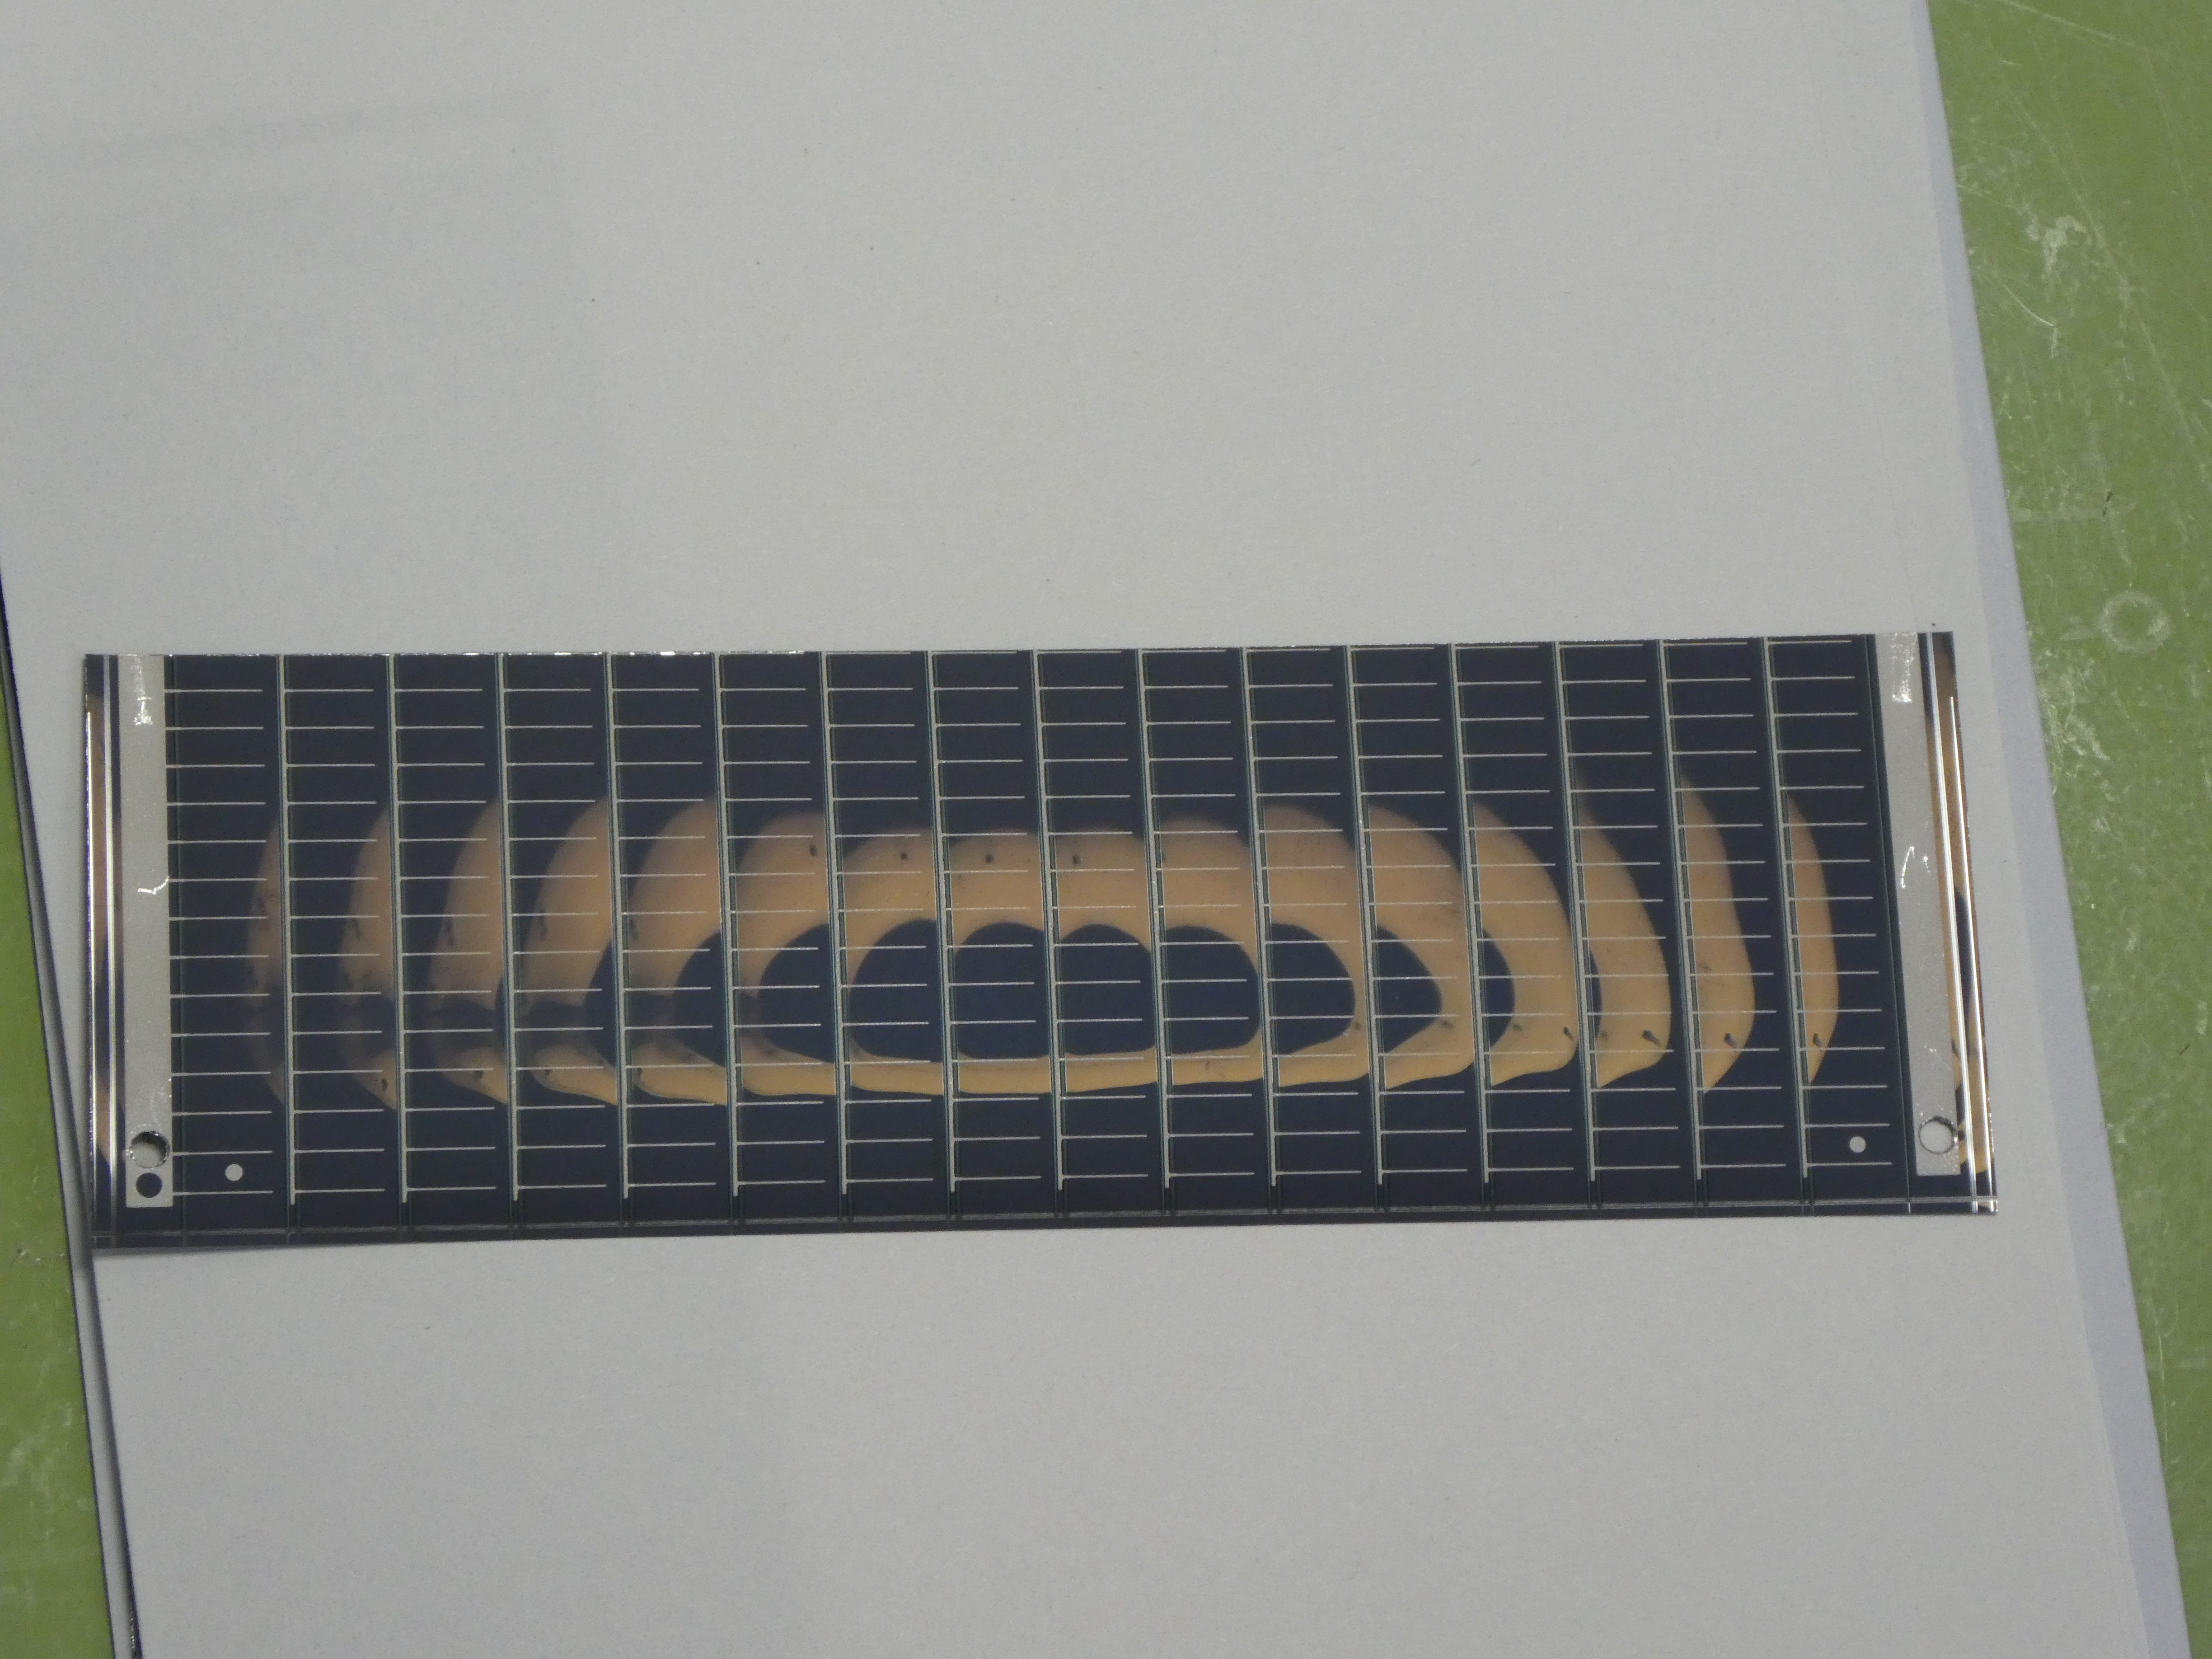
\includegraphics[scale=0.1]{03/fig/makeTFSC_TFSC.jpg}
		\caption{ねじ留め用の穴を開けた薄膜太陽電池}
		\label{fig3-9-3-3}
	\end{figure}
	\item[\textbf{2.半田付けをする}]
	サーミスタと電極にそれぞれフレキシブル導電糸を半田付けする.サーミスタは半田部分に熱収縮チューブを取り付ける.また,サーミスタははんだ耐熱性が決まっている(260℃,5秒)ので,注意する.電極は薄膜太陽電池の両端でそれぞれ向きが異なるので注意する.
	\begin{figure}[H]
		\begin{tabular}{cc}
			\begin{minipage}[t]{0.45\hsize}
				\centering
				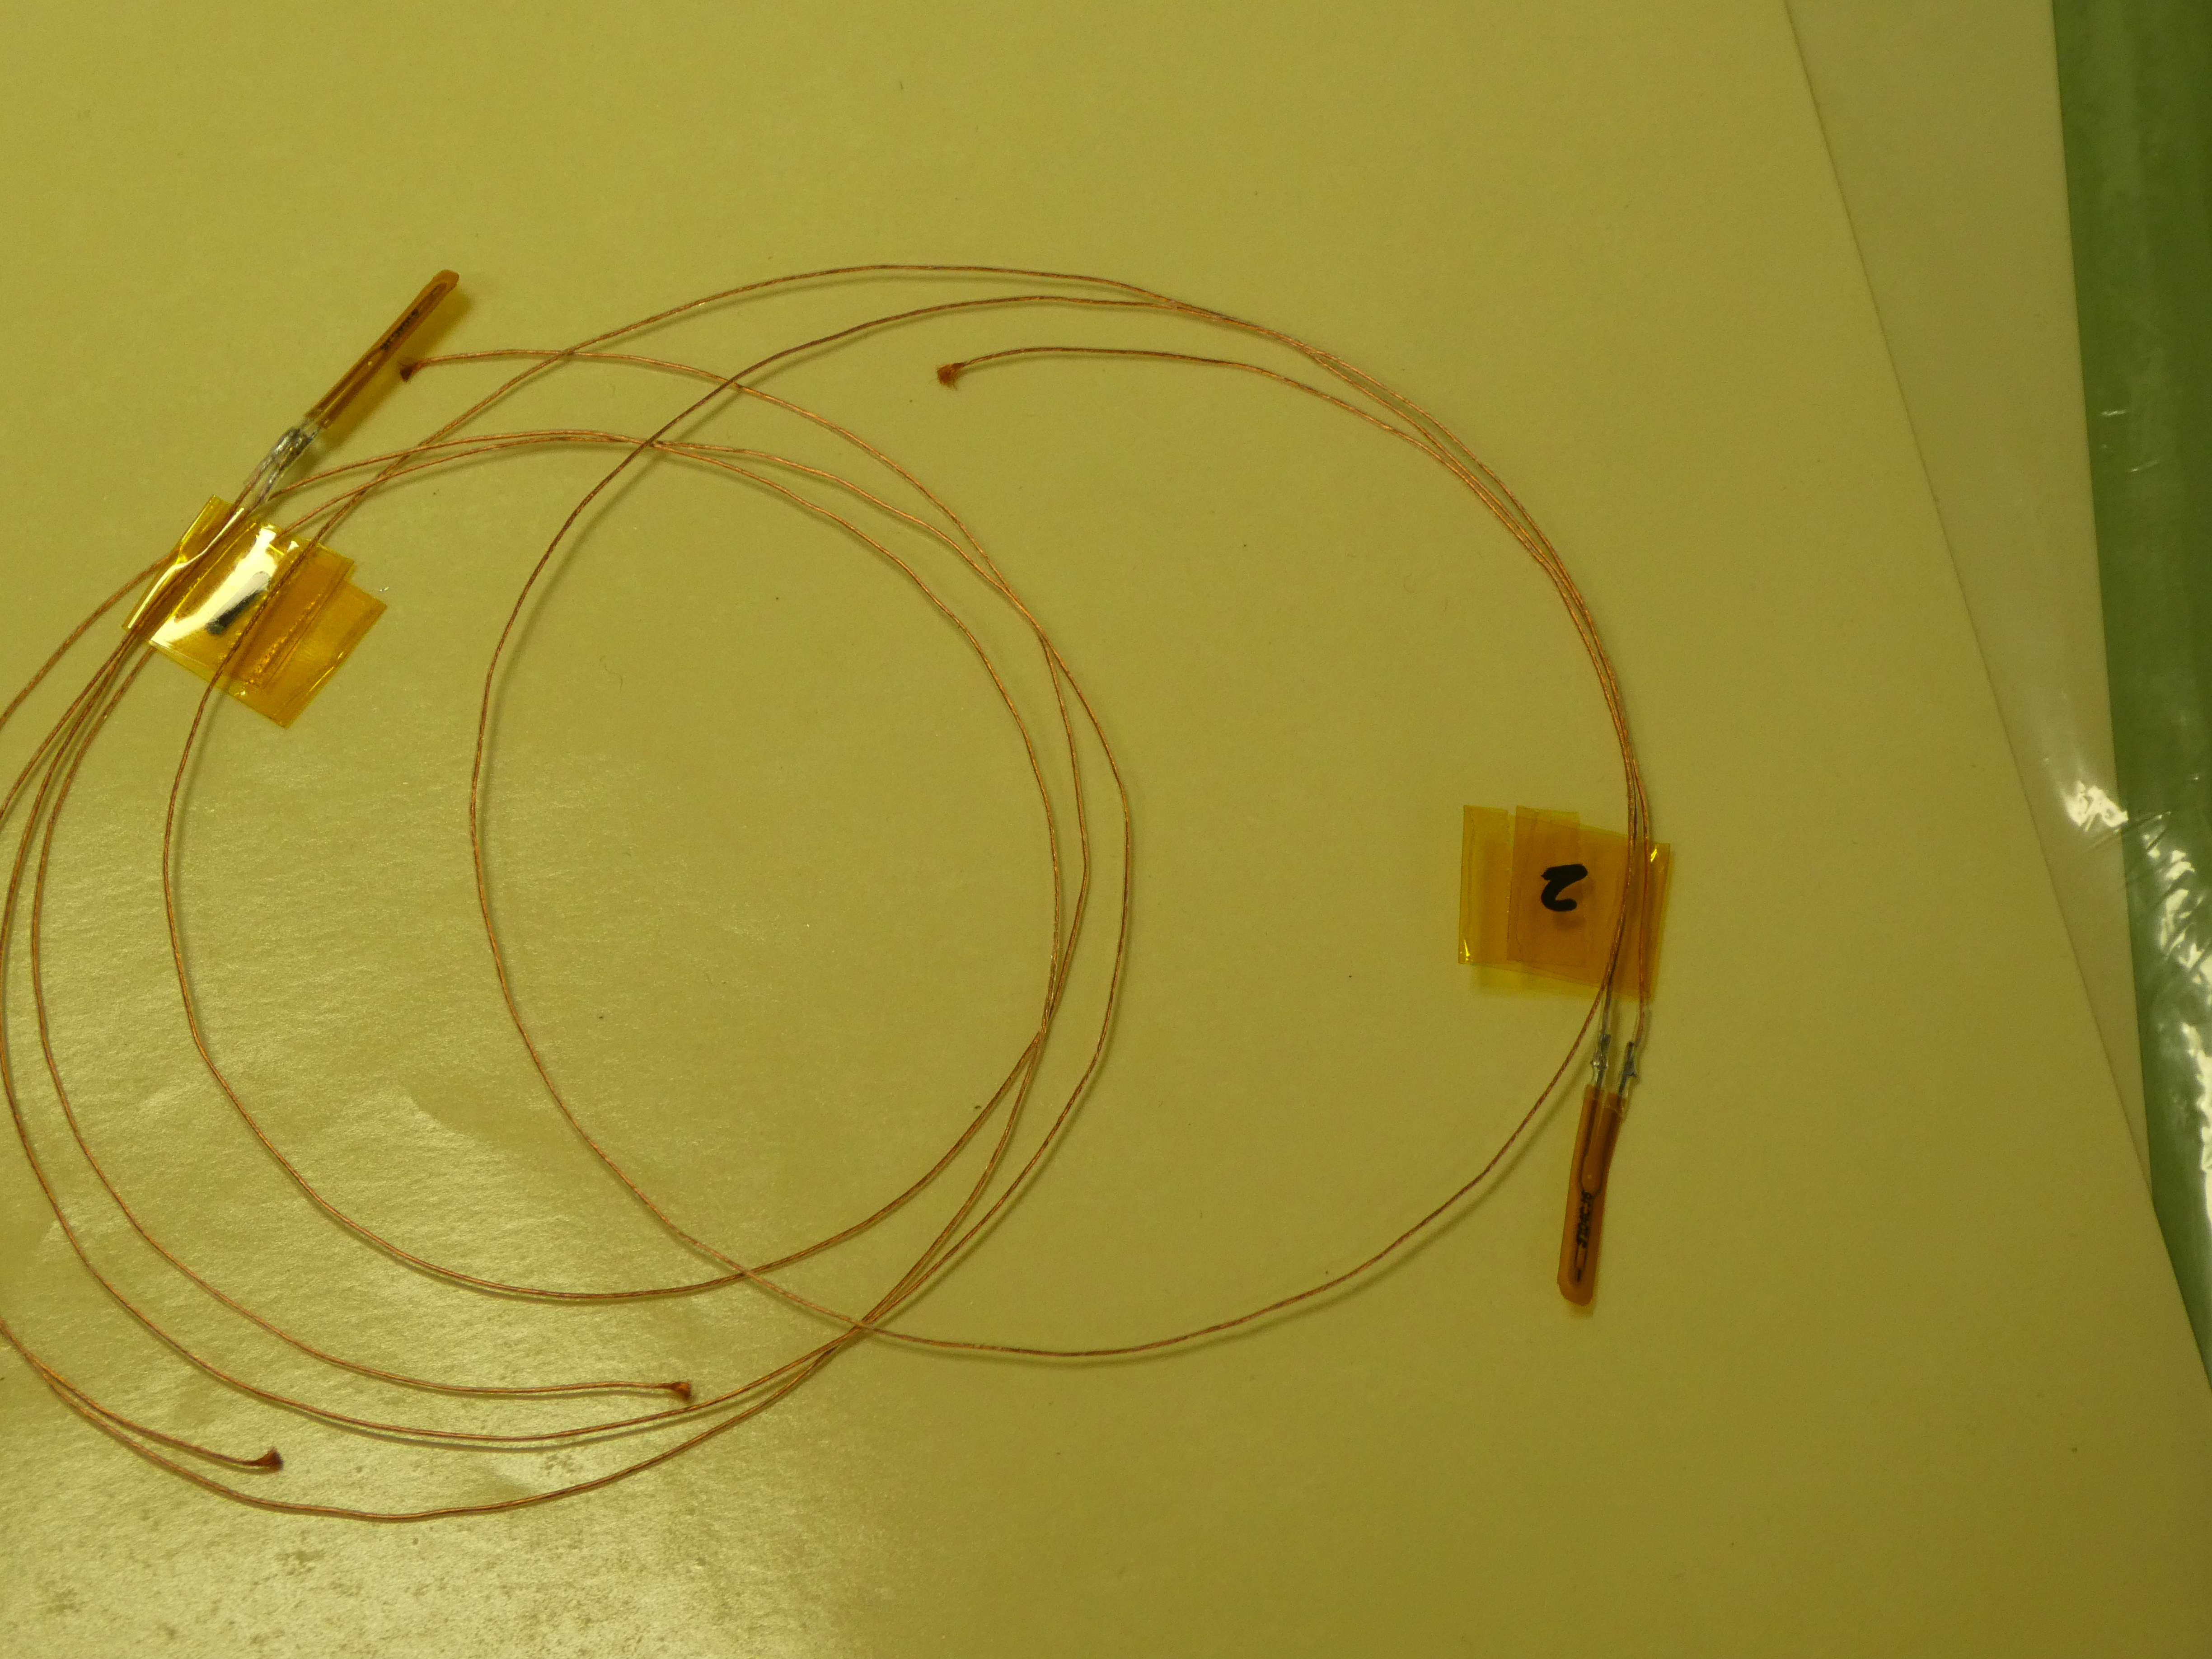
\includegraphics[scale=0.07]{03/fig/makeTFSC_thrm.jpg}
				\caption{はんだ付けしたサーミスタ}
				\label{fig3-9-3-4}
			\end{minipage} &
		
			\begin{minipage}[t]{0.45\hsize}
				\centering
				\includegraphics[scale=0.35]{03/fig/makeTFSC_harn.jpg}
				\caption{はんだ付けした電極}
				\label{fig3-9-3-5}
			\end{minipage}
		\end{tabular}	
	\end{figure}
	\item[\textbf{3.フレキシブル導電糸を薄膜太陽電池に固定する}]
	電極を,PEEKねじで固定する.トルク値は0.03N・m(推奨締め付けトルク).基板側の導電糸の先端にどの太陽電池の導電糸かわかるようにナンバリング等を行うことに気をつける.展開膜収納後,たくさんあるハーネスの中で区別がつくようにしないと基板側との接続ができなくなる.
		\begin{figure}[H]
		\begin{tabular}{cc}
			\begin{minipage}[t]{0.45\hsize}
				\centering
				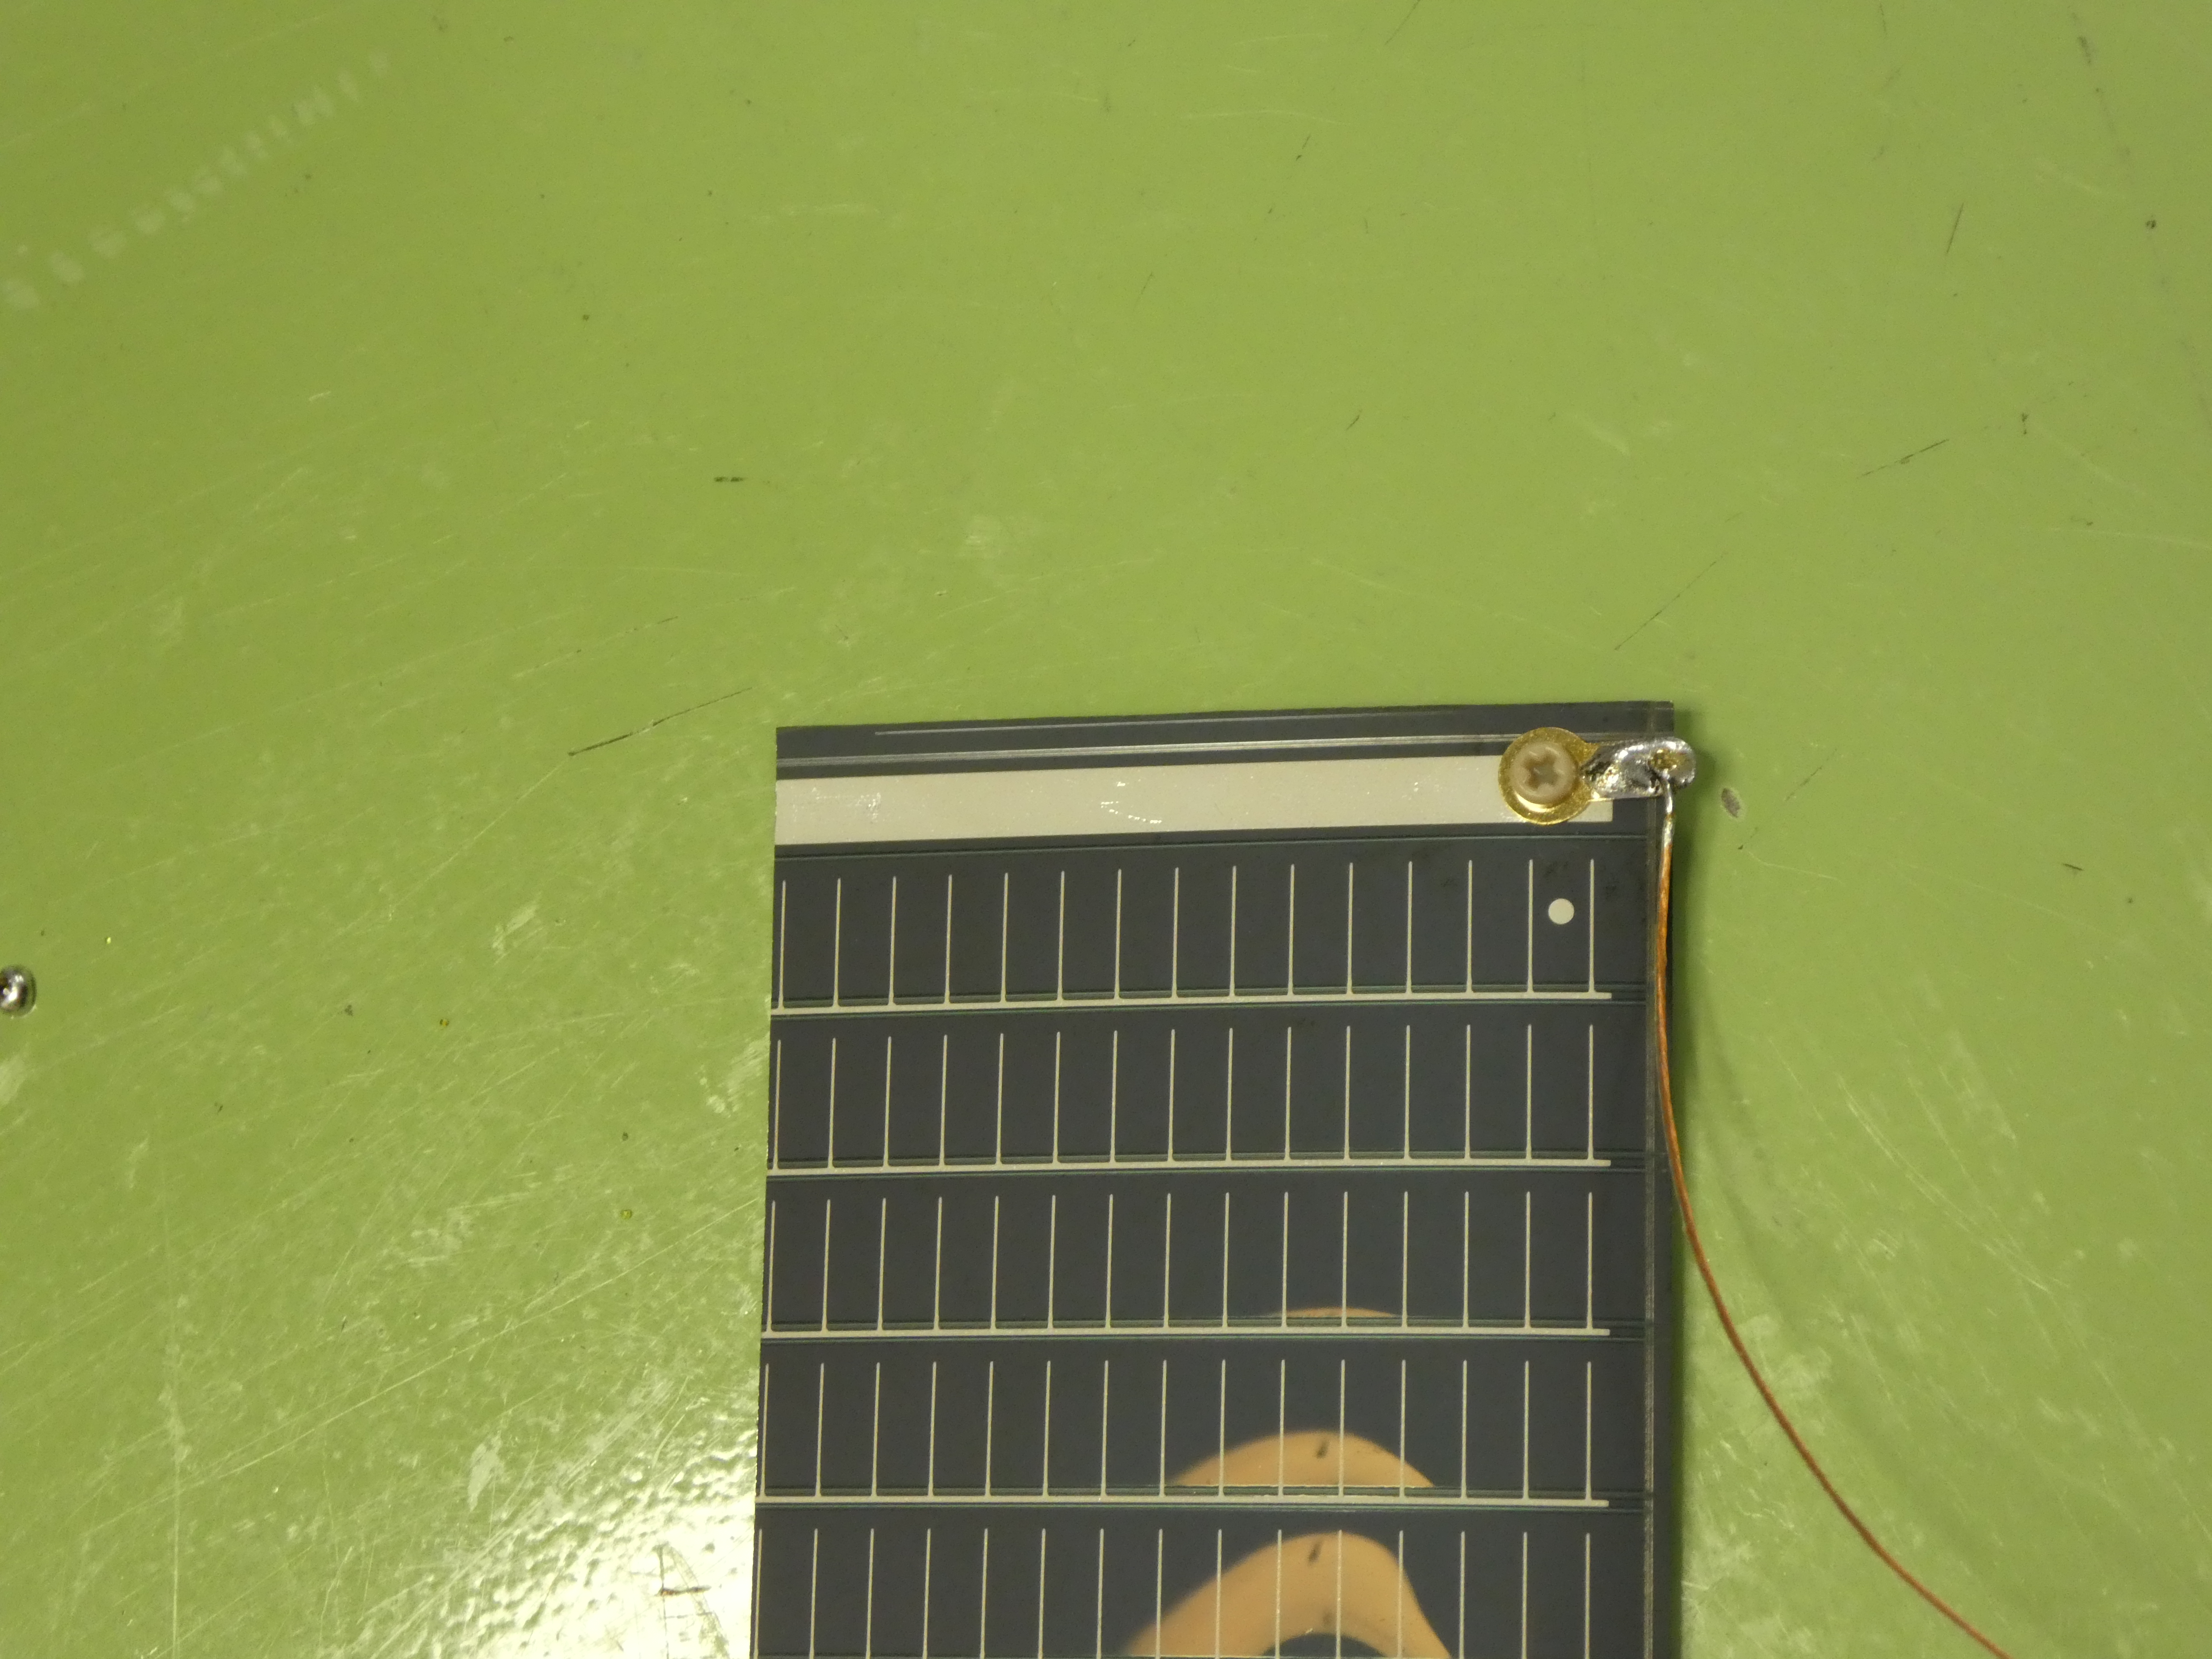
\includegraphics[scale=0.07]{03/fig/makeTFSC_harn-TFSC_1.jpg}
				\caption{ねじ留めした薄膜太陽電池(外側)}
				\label{fig3-9-3-6}
			\end{minipage} &
			
			\begin{minipage}[t]{0.45\hsize}
				\centering
				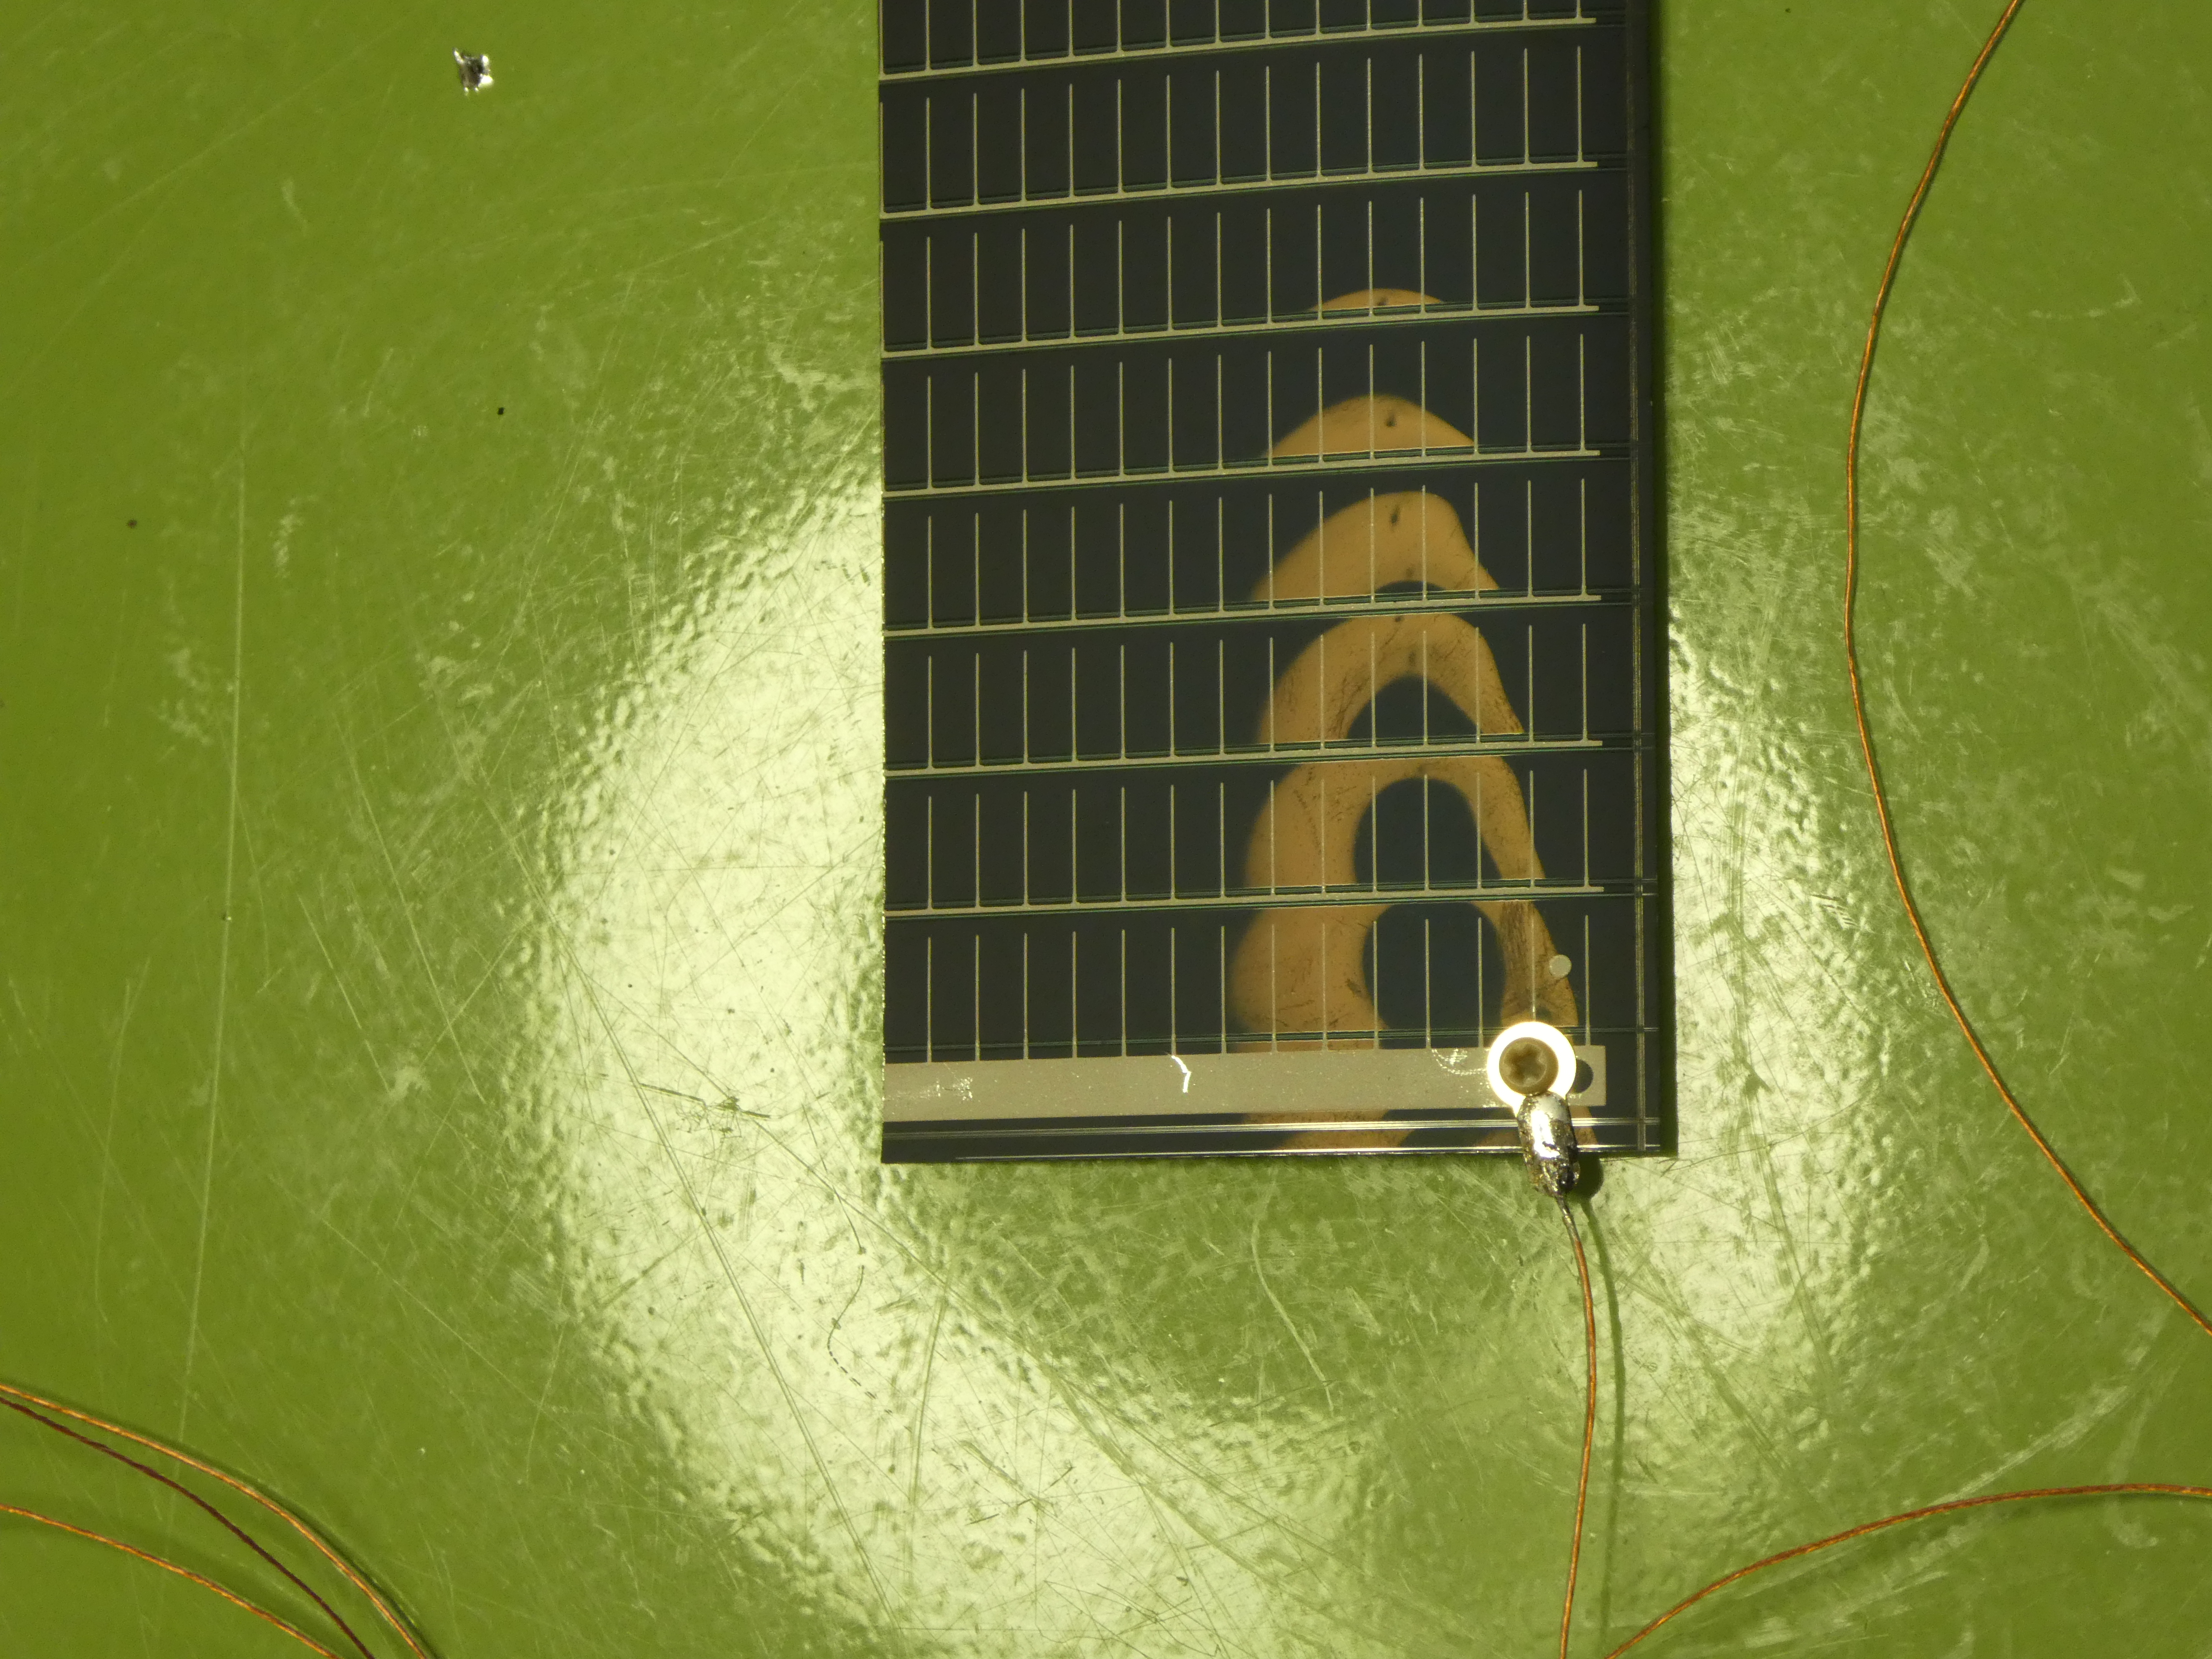
\includegraphics[scale=0.07]{03/fig/makeTFSC_harn-TFSC_2.jpg}
				\caption{ねじ留めした薄膜太陽電池(内側)}
				\label{fig3-9-3-7}
			\end{minipage}
		\end{tabular}	
	\end{figure}
	\item[\textbf{4.サーミスタを接着する}]
	サーミスタにホットメルト接着剤を貼付し,アイロンで熱癒着させる(100℃,10秒).その後,薄膜太陽電池に熱癒着させる(100℃,10秒).基板側の導電糸の先端にどちらの太陽電池のサーミスタかわかるようにナンバリング等を行うことに気をつける.
	\begin{figure}[H]
		\begin{tabular}{cc}
			\begin{minipage}[t]{0.45\hsize}
				\centering
				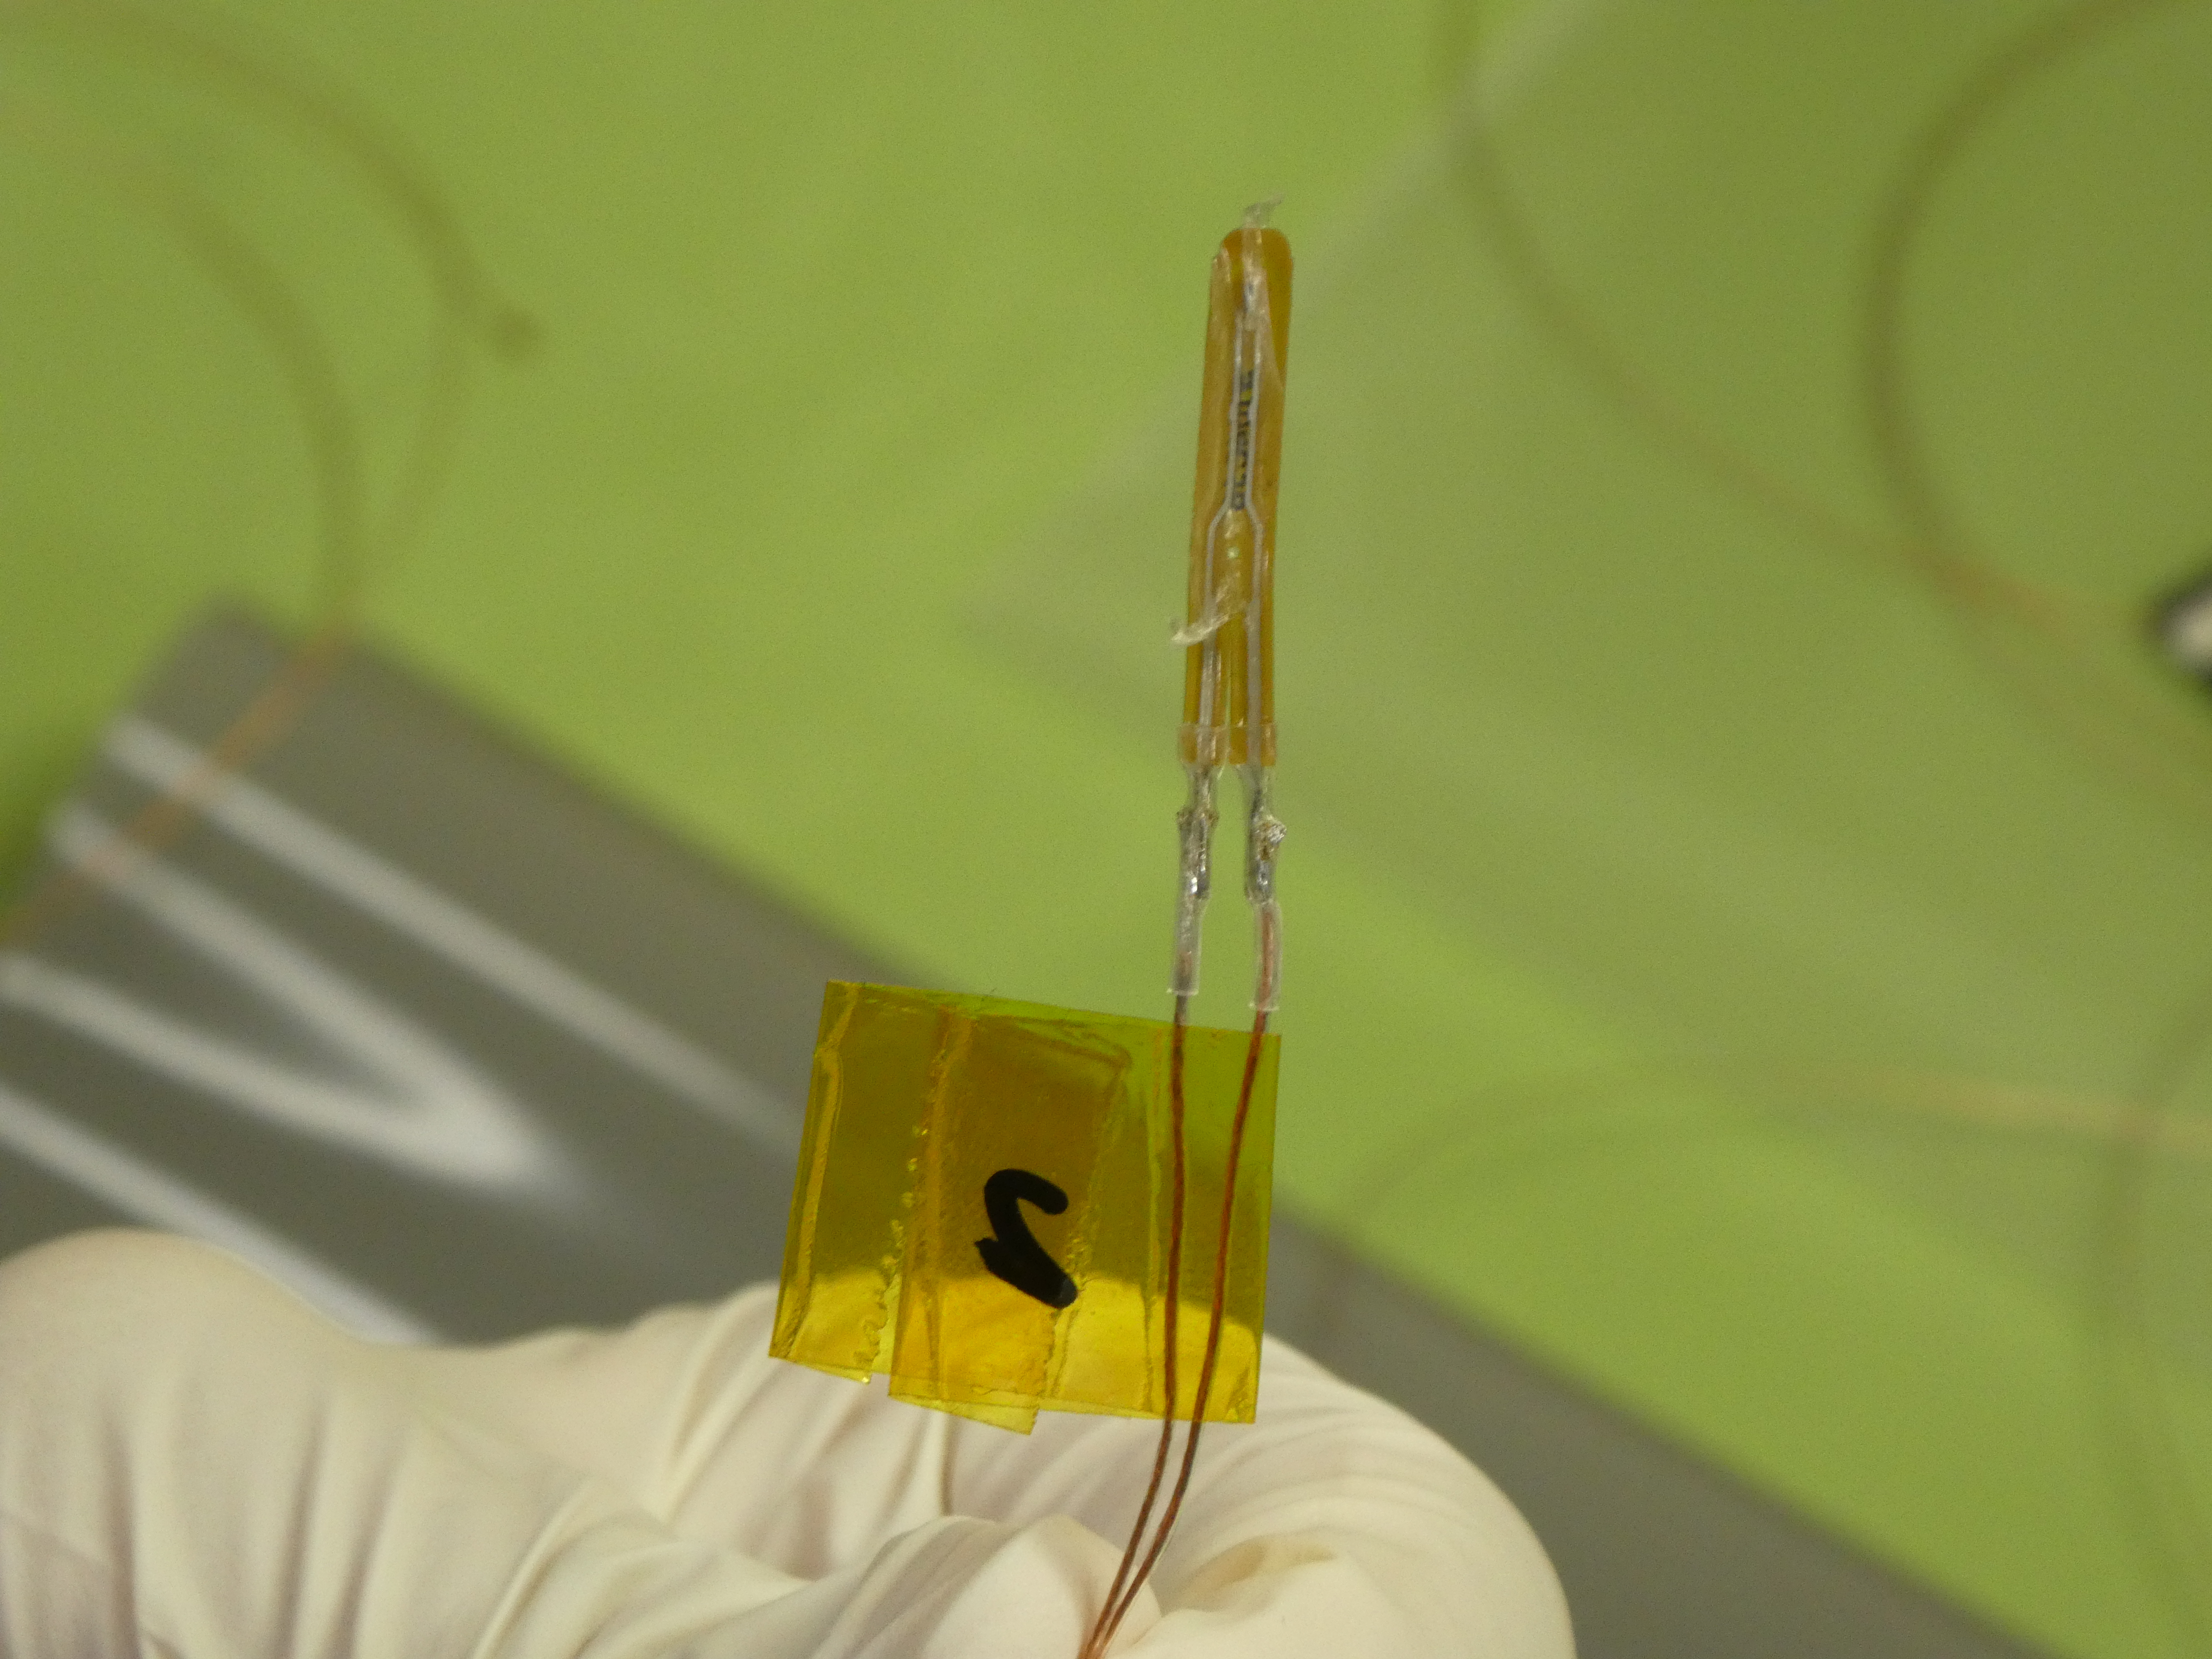
\includegraphics[scale=0.07]{03/fig/makeTFSC_thrm-adhe.jpg}
				\caption{ホットメルト接着剤を貼付したサーミスタ}
				\label{fig3-9-3-8}
			\end{minipage} &
			
			\begin{minipage}[t]{0.45\hsize}
				\centering
				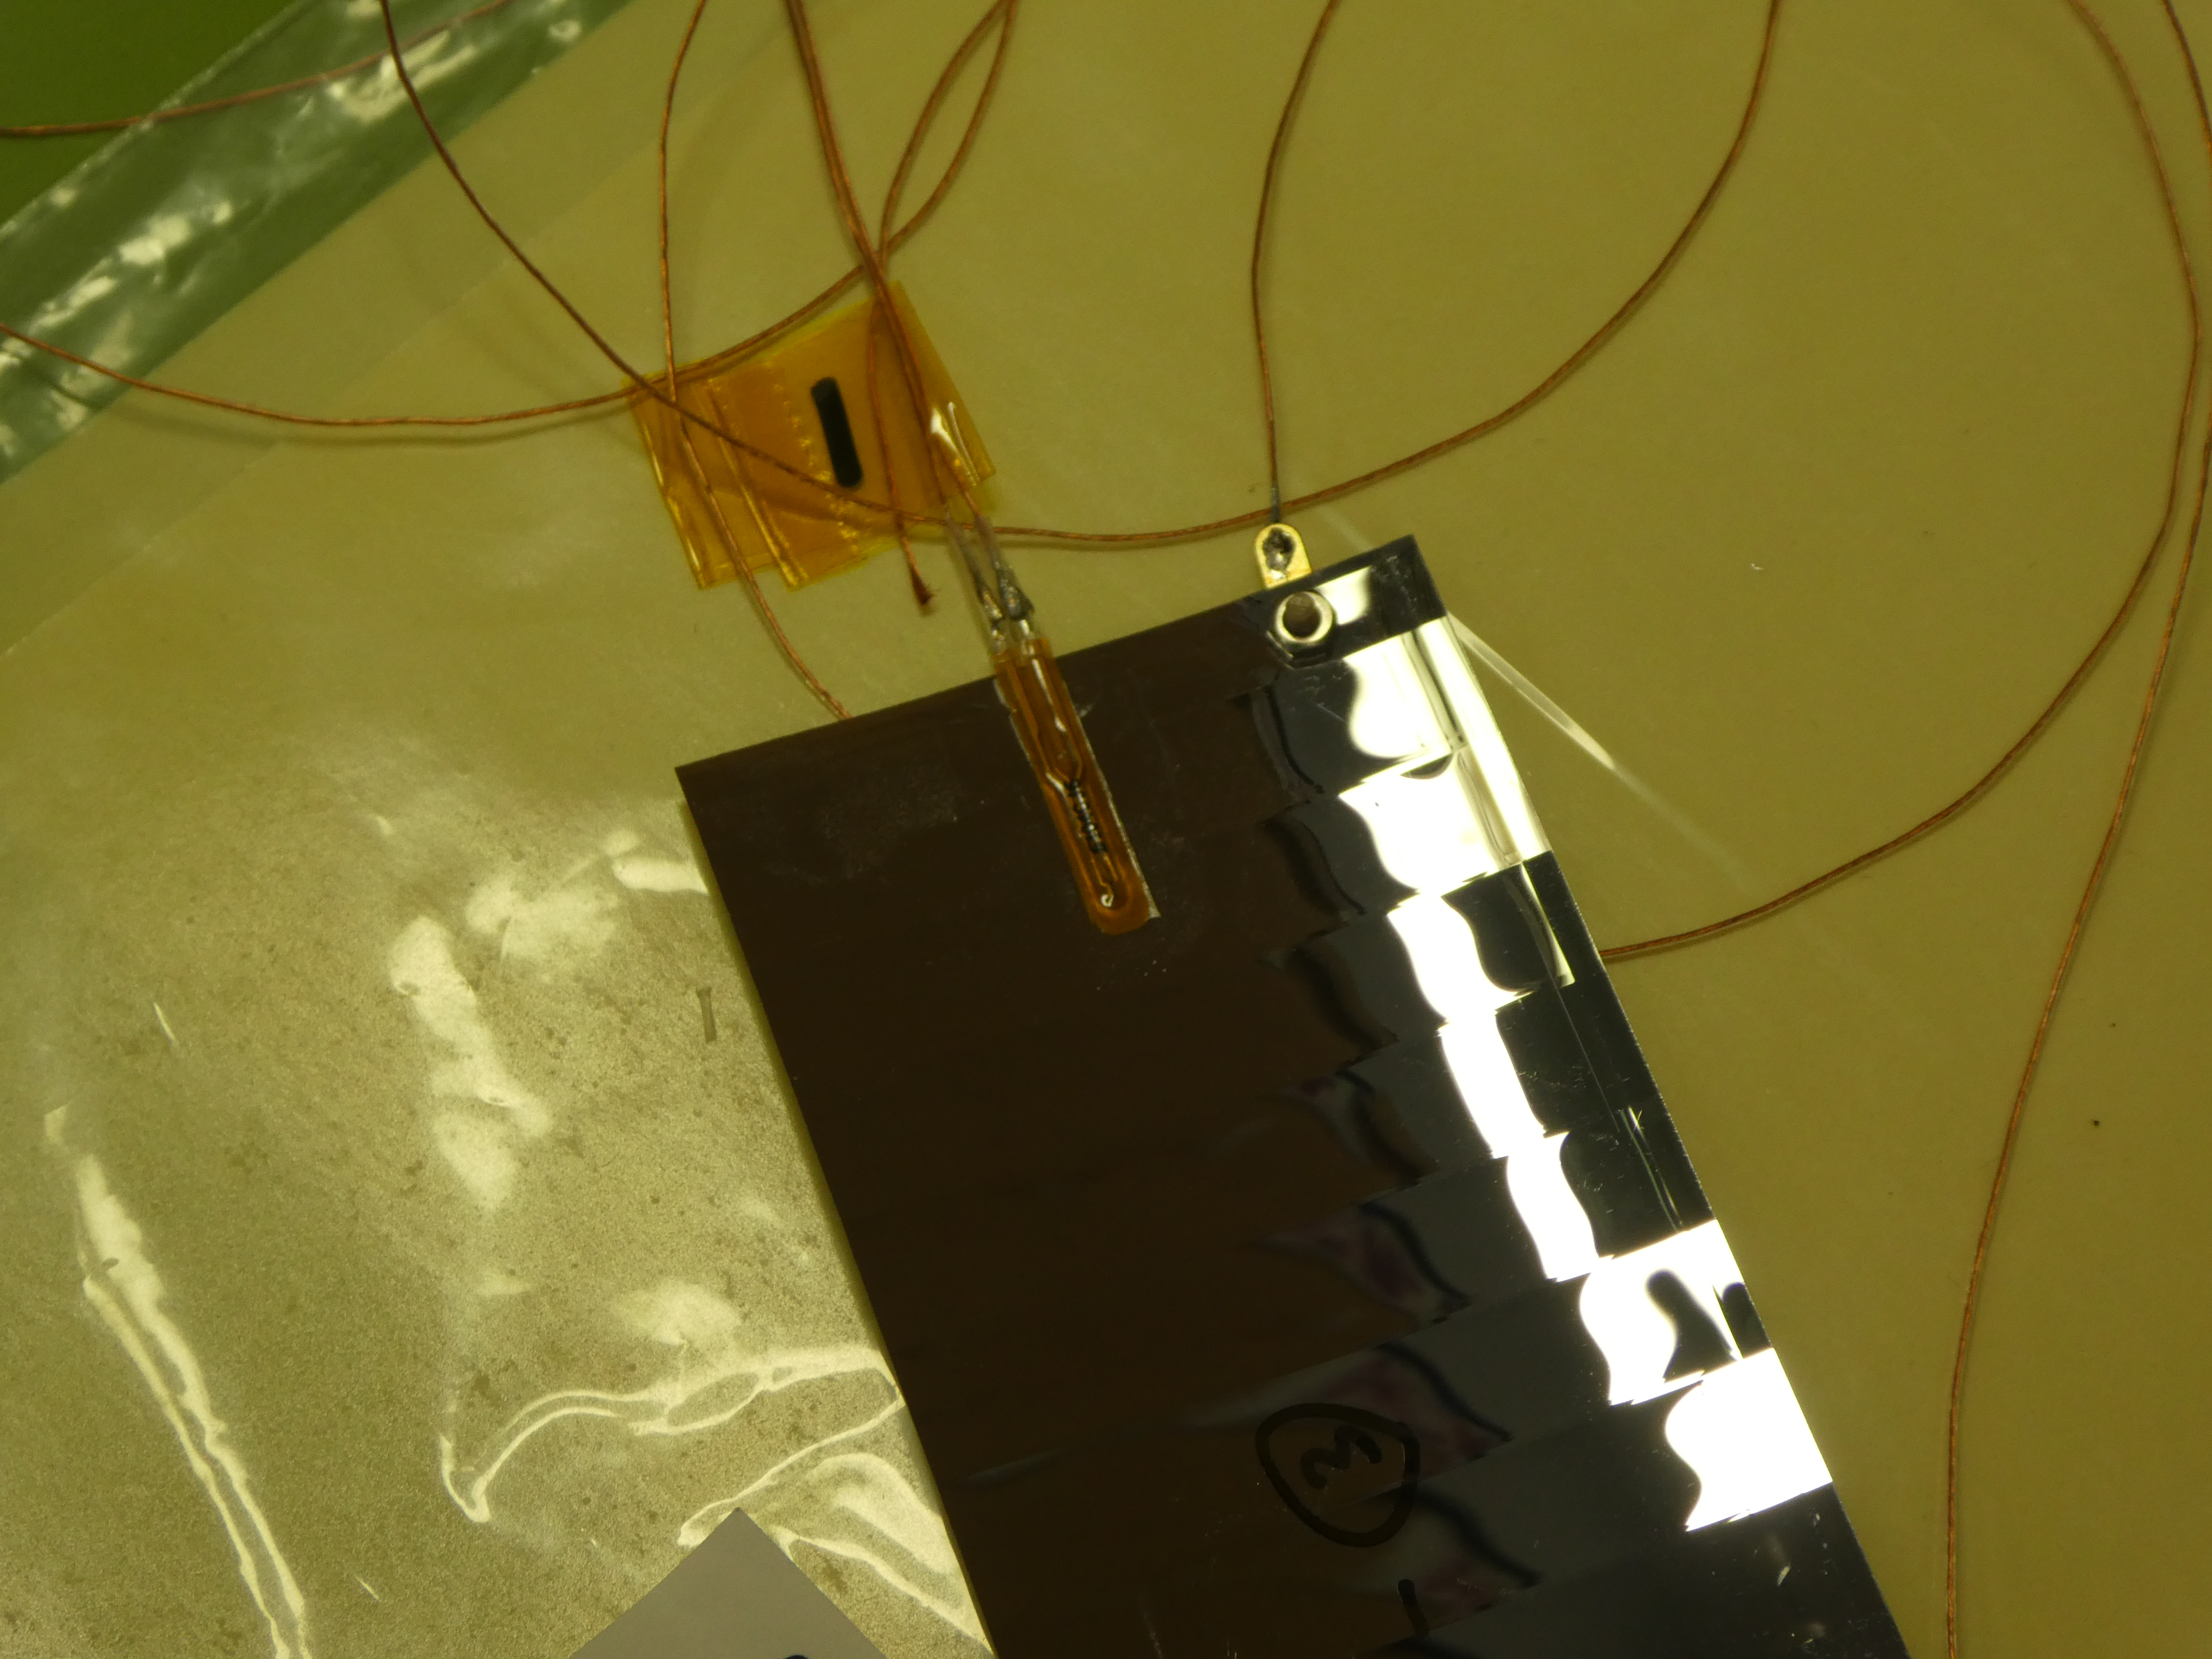
\includegraphics[scale=0.07]{03/fig/makeTFSC_thrm-TFSC.jpg}
				\caption{サーミスタを貼付した薄膜太陽電池}
				\label{fig3-9-3-9}
			\end{minipage}
		\end{tabular}	
	\end{figure}
	\item[\textbf{5.薄膜太陽電池を展開膜に接着する}]
	図\ref{fig3-9-3-10}に表せられたようにホットメルト接着剤(1cm角)を貼付し,アイロンで熱癒着させる(100℃,10秒).接着後,展開膜に同様に接着する.
	\begin{figure}[H]
		\centering
		\includegraphics[scale=0.4]{03/fig/makeTFSC_TFSC-mem.jpg}
		\caption{ホットメルト接着剤を貼付した薄膜太陽電池}
		\label{fig3-9-3-10}
	\end{figure}
	\item[\textbf{6.フレキシブル導電糸を展開膜に配線する}]
	図\ref{fig3-9-3-11}のとおりに配線する.
	\textbf{
		\begin{figure}[H]
			\centering
			\includegraphics[scale=0.4]{03/fig/makeTFSC_harn_make.jpg}
			\caption{配線方法}
			\label{fig3-9-3-11}
		\end{figure}
	}
	\item[\textbf{完成}]
\end{itemize}

\subsubsection*{薄膜太陽電池の管理方法}
ナンバリング等できちんと管理する.発電特性の実験をしたらどの薄膜太陽電池のものかわかるように管理する.

